\section{Implementation Architecture}

\subsection{Introduction}
Divide and conquer. How better to describe Information Technology than by this concept?
We therefore have to divide the code into different parts in order to better frame 
the problem and be able to solve it. In order to take control of the car, we decided 
to implement a control-observer architecture. This architecture divides the project 
into different parts and thus partitions the code. To implement this architecture, we
can use a middleware like the \textit{Robot Operating System} (ROS) which will allow us
to simplify the communication between the different sectors through messages.

\subsection{Overview} % Not the right word I think

\begin{figure}[!ht]
    \begin{center}
        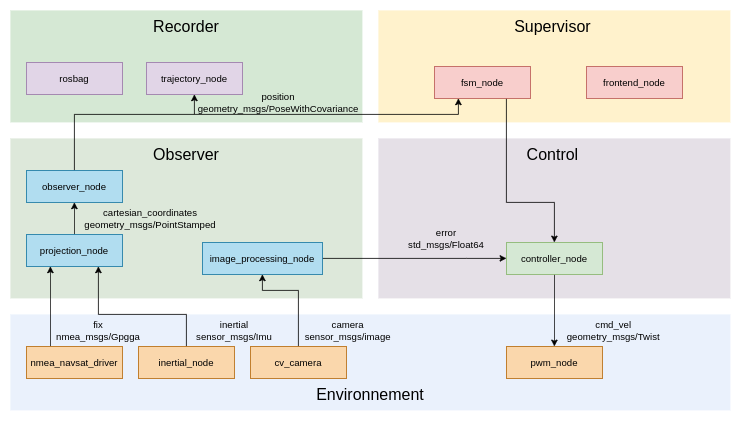
\includegraphics[scale=0.51]{Images/node_graph.png}
    \end{center}
    \caption{Implementation Architecture of this project}
    \label{fig:node_graph}
\end{figure}

\textbf{Figure}~\ref{fig:node_graph} represents the implementation architecture of our project.
In classical architectures, there are five main sections: Environment, 
Observer, Control, Recorder and Supervisor. They are then present in the architecture 
of our project. 

\paragraph{Environment} This section gathers all the low level nodes allowing the 
communication with the hardware. This entire section can be replaced by a simulation
node that would publish the same messages in order to evaluate the rest of the 
functional architecture. In this project we have a global navigation satellite system
(GNSS), an inertial unit and a camera. Finally we can control the speed of the rear
engine and the position of the servomotor steering the car.

\paragraph{Observer} This section is used to process data from the different sensors of
the robot. In particular, it will be used here to perform image processing on the data
from the camera. It will also allow to merge the data from the inertial unit and the GNSS
in a Kalman filter to estimate more precisely the position of the car.

\paragraph{Control} This section allow us to establish several control laws for our robot
from the sensor data in order to drive our car's actuators. The Supervisor section will
indicates the right control law on a case-by-case basis.

\paragraph{Recorder} This section records the various robot data in order to be able to 
replay the data, particularly through rosbags, and it records the trajectory of the robot
to feed the finite state machine.

\paragraph{Supervisor} This section consists mainly of the finite state machine that controls
the mission. It will determine the right command law to control the robot according to what the
robot can perceive from its environment. There is also a front-end server that allows us to have
a feedback, a graphical user interface to know the state of the robot.

\newpage